\documentclass[11pt,report]{jsarticle}
\usepackage[dvipdfmx]{graphicx}
\usepackage{wrapfig}
\usepackage{float}
\usepackage{otf}
\usepackage{longtable}
\usepackage{ulem}
\usepackage{ascmac}
\usepackage{url}                                                                                                                                                                                                                                                                                                                      
%%%%%
\setlength{\textwidth}{160truemm}      % テキスト幅: 160mm
\setlength{\fullwidth}{\textwidth}     % ページ全体の幅
\setlength{\oddsidemargin}{0mm}   % 左余白
\setlength{\topmargin}{-15mm}       % 上余白
\setlength{\textheight}{250truemm}     % テキスト高さ: 297-(30+30)=237mm
\title{箱館戦争戦跡の考古学的調査 \\ \Large{二股台場の測量調査}} % 文書のタイトル
\date{2019年12月7日}
\author{箱館戦争戦跡調査プロジェクト \\石井淳平,野村祐一,塚田直哉,時田太一郎}              % 著者

%%%%
\begin{document} 
\maketitle
%%%%
\begin{abstract}
明治2年の箱館戦争に際して構築されたと伝えられる北斗市二股台場の全面的な踏査と測量調査を行ったので、その結果を報告する。各塹壕の配置や可視領域の分析によって、複数の塹壕が連携して一定の機能を果たしていたことが明らかとなった。同一機能を有する塹壕群単位に塹壕を再編成した結果、二股台場は施条銃を用いた戦闘様式に基づいて、正面防御と側面射撃は組み合わせた合理的な野戦築城が行われたと評価した。
\end{abstract}

%%%%
\section{はじめに}
北海道の南西部、北斗市山中の台場山に、「二股台場」(北海道教育委員会埋蔵文化財包蔵地「台場山遺跡」(B-06-102))として知られる塹壕群が残されている。これらの塹壕は、明治2年(1869)の戦いで旧幕府軍が構築したと伝えられている。箱館戦争の戦跡としてだけではなく、城郭史研究の視点からも重要な遺跡である。

本調査ではこれまで知られている台場山周辺の塹壕群の測量を行い、塹壕群の形状と位置の記録を行った。2018年と2019年の調査において、既知の18箇所の塹壕跡のうち確認できた11箇所と新発見の塹壕跡2箇所の測量調査を実施した。

%%%%
\section{明治2年箱館戦争と二股台場の位置}
\subsection{明治2年箱館戦争}

\begin{figure}[ht]
\centering
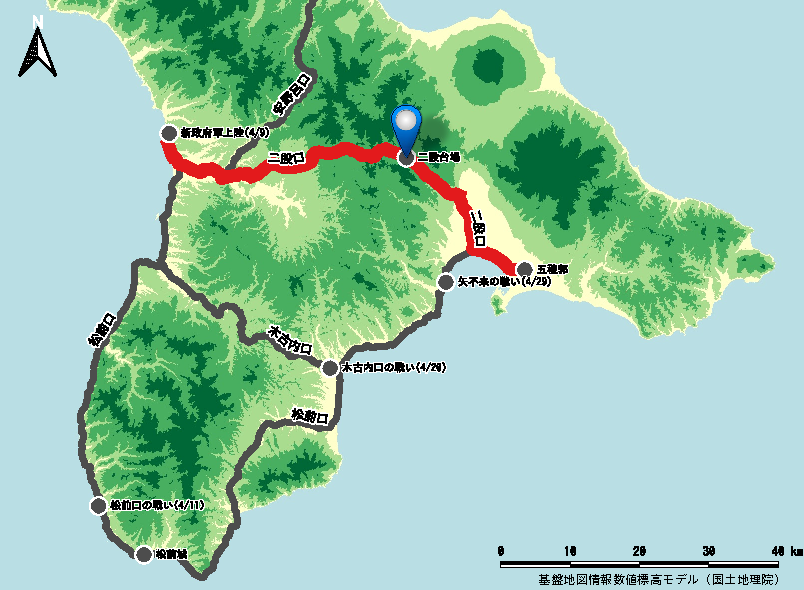
\includegraphics[width=160truemm]{../02fig/01dounan_map.pdf}
\caption{明治2年箱館戦争と二股台場の位置}
\label{dounan_map}
\end{figure}

明治2年4月9日、旧幕府軍に占領された蝦夷地奪還のため、新政府軍は北海道南西部の乙部に上陸した。新政府軍の攻撃軸は松前口、二股口、安野呂口の3本が設定され、南蝦夷地の要衝である江差、松前を経て箱館へ至る松前口とそこから分岐した木古内口に最大の兵力が割かれた。二股口は松前口に次ぐ兵力が派遣された(図\ref{dounan_map})。二股口は険しい山道の進軍を余儀なくされるが、強固な防御拠点もなく、兵力に乏しい旧幕府軍兵力の分断と各個の突破を図ったものと考えられる。

\subsection{二股台場の位置}

\begin{figure}[ht]
\centering
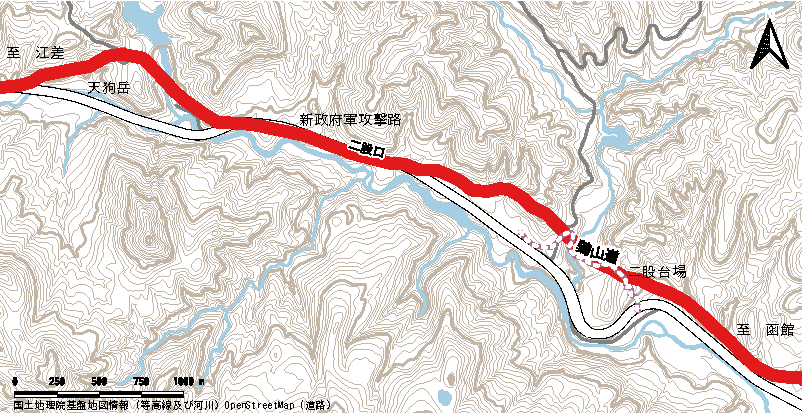
\includegraphics[width=160truemm]{../02fig/02futamata_map.pdf}
\caption{二股台場周辺の地形}
\label{futamata_map}
\end{figure}

二股台場は北斗市大野町市街地から北西約10km上流の大野川左岸、大野川とその支流である二股沢川の合流点付近に位置する(図\ref{futamata_map})。大野市街地から二股沢川付近までは大野川に沿って平坦な地形が続くが、二股台場塹壕群の所在する尾根を境に、これより上流では尾根と谷が交互に現れる急峻な地形となる。

二股台場塹壕群は標高261mの台場山と、これと一連の尾根をなす339m峰との間の尾根上に確認されており、二股沢川にと並行に北方から大野川にむかって傾斜する尾根上に塹壕群が並ぶ。最高地点に立地する塹壕(F15)は標高約330m、最低地点に立地する塹壕(F16)は約200mである。尾根の鞍部を旧道である「鶉山道」が横切っており、塹壕群は鞍部をはさんで南北に分かれる。

新政府軍の攻撃正面となった尾根の西側斜面は鶉山道南側では平均傾斜約20度、鶉山道北側では約30度である。

%%%%
\section{文献からみる二股台場の戦い}
\subsection{概要}
二股台場の戦いについての文献記録は、旧幕府軍側・新政府軍側を併せ数多く残るが、両軍記録ともに自軍視点での記述に偏りがちである。旧幕府軍側は対陣した新政府軍側の陣容に不正確な点が見られ、また戦果についても過大評価のきらいがある。また新政府軍側は各藩の出陣記録が主であり、個別詳細については事実に近しいものの、軍の全容についての総合的な記述に乏しい。

以下は、それらを総見・整理し、二股台場の戦いにおける両軍の陣容および戦闘経過についての整合・把握を試みたものである。文献出典は適宜括弧書きにして記載する(1)(括弧中[幕]は旧幕府軍側文献、[新]は新政府軍側文献)。

%%%
\subsection{新政府軍の乙部上陸から二股口進撃まで}
明治2(1869)年4月6日(新暦5月14日)、新政府軍は青森を進発し、4月9日(新暦5月17日)、乙部に上陸。軍を二手に分け、一方は海岸より松前方面、うち一方は江差より山中を抜き函館平野・五稜郭へ攻め入るべく進軍を開始する([新]『戦争御届書』(松前藩)『戊巳征戦記略』(長州藩)『阿部正桓家譜』(福山藩))。この時の新政府軍の陣容は以下の通り。

\begin{description}
\item [松前藩] 1中隊(一番小半隊・二番厚田清隊からなる中隊)総長・松前右京、軍事方・松崎多門(『戦争御届書』)
\item [長州藩] 2中隊+半砲隊(第二中隊・第三中隊・第二半砲隊)軍監・駒井政五郎(『戊巳征戦記略』)
\item [福山藩] 2中隊+砲隊(一番中隊・三番中隊・砲隊)副総督・堀兵左衛門、軍監・関新五左衛門(『阿部正桓家譜』)
\end{description}

幕末当時の軍制に照らし合わせおおよそ500から600名の陣容となり、これは二股台場において新政府軍を迎え撃った旧幕府軍側の記録における見立てと合致する([幕]『南柯紀行』『説夢録』『北洲新話』『戊辰戦争見聞略記』『函館戦記』)。

新政府軍進撃の報は4月9日のうちに五稜郭の旧幕府軍本陣にもたらされ([幕]『中島登覚え書』『函館戦記』『衝鋒隊戦争略記』)、これを迎え撃つべく、旧幕府軍は間道途上・二股の地に軍を進め、4月12日までの間に迎撃のための胸壁(塹壕)を築く(『北洲新話』には「春来築きしもあり」との記述もある)。これが、現在も遺る現・台場山の塹壕群である。

この際築かれた胸壁の数については、旧幕府軍側の文献のうち『蝦夷之夢』『北洲新話』『蝦夷錦』『函館戦記』にあるがいずれも16か所である。種別詳細について記録があるのはこのうち大野右仲の『函館戦記』であるが、それによれば「山巓と半腹とに築くものは十一。河岸に築くもの三。広くして大なるもの二。道を挟んで築き、昼夜督役せしかば二日にして成る」「伝習歩兵隊をして右の山の諸壁を守らしめ、衝鋒隊をして左の山と河岸とを守らしむ」とある。また新政府側の戦闘記録中にも「左右山手」(『津軽承昭家記』(弘前藩))「左半隊ハ山手右道ヲ相固、右半隊ハ正面ニ相懸…」(『薩摩出軍戦状』(薩摩藩))など、道即ち旧間道を挟む台場山の高峰・低峰に分散して塹壕が築かれていたと読みとれる箇所があり、これは現在既知の山嶺上の遺構分布と合致する。ただし大野の記述における「河岸に築くもの三」「広くして大なるもの二」、『蝦夷之夢』『函館戦記』における第二次会戦の戦闘中に新政府軍に奪取された山嶺塹壕と河岸の兵とに旧幕府軍の塹壕が挟み撃ちを受ける描写などから見えるように、山嶺塹壕のほか二股河岸にも塹壕が構築されていた可能性が高いが、こちらについては未発見である。

旧幕府軍はこのほか、「官軍の動静を伺はす」([幕]『函館戦記』)ために下二股よりおよそ一里にある「天狗岩」にも胸壁を築いた。この際築かれた壁数については、旧幕府軍側記録には3か所(『函館戦記』)ないし4か所(『蝦夷之夢』『北洲新話』)の2通りの記録がある。なお、新政府軍側・長州藩の『戊巳征戦記略』には「…中二股ノ賊壘三所ヲ撃破シ…」との記録がある。また「天狗岩」の現在地についてであるが、おそらくは現在の北斗市に所在する天狗岳が該当すると考えられるが、松前藩の記録では「天狗嶽(岳)より八・九町隔てた『三枚嶽』と申す山の半腹」(『戦争御届書』)とあることを付記しておく。
これらの胸壁群を守った旧幕府軍の初期陣容については、凡そ以下の通りである。

\begin{description}
\item [陸軍奉行並] 土方歳三(市ノ渡宿陣)
\item [同 添 役] 大野右仲、大島寅雄(出陣時、開戦時は五稜郭に)
\item [陸軍改役下役] アルテュール=フォルタン
\item [衝鋒隊]	二小隊(頭取・友野栄之助・川井卓郎(卓太郎)、指図役・小和野昌太郎)
\item 伝習歩兵隊] 一小隊(頭取・中根量三)
\item [砲兵隊]
\item [工兵隊] (隊 長・吉沢勇四郎)
\end{description}

これを幕末軍制に照らせば、『衝鋒隊戦争略記』『函館戦記(大野版)』における「百三十人余」という兵数とおおよそ合致する。この2文献は実際に二股口防戦にあたったメンバーの聞き取りあるいは実録によるものであり、信憑性も比較的高いものと考えられる。

%%%
\subsection{天狗岩の前哨戦と第一次会戦(旧暦明治2年4月13日~14日)}
4月13日(新暦5月24日)午後3時ごろ([幕]『北洲新話』『函館戦記』)、長州藩・福山藩・松前藩が天狗岩の旧幕府軍陣地へ襲来([新]『戊巳征戦記略』『阿部正桓家譜』『戦争御届書』)。天狗岩に新政府軍迫るの報はすぐさま後陣・下二股台場へと伝わり、北側峰の胸壁群には伝習歩兵隊、南側峰と河岸の胸壁群には衝鋒隊が伏せ来襲に備える([幕]『衝鋒隊戦争略記』『函館戦記』)。

このとき土方歳三は市渡に宿陣していた([幕]『中島登覚え書』『函館戦記』)ため、報せの早馬が発せられ([幕]『函館戦記』)、これを受けて土方もすぐに出陣、指揮にあたる([幕]『島田魁日記』)。

新政府軍は、主力が天狗岩陣地正面から攻撃するところを長州藩の別働隊が山上から回り込み旧幕府軍を挟撃([新]『戦争御届書』(松前藩)『阿部正桓家譜』(福山藩)[幕]『北洲新話』)、同地の胸壁3ヶ所は全て陥落する([新]『戊巳征戦記略』(長州藩)など)。旧幕府軍は撤退すると同時に、新政府軍を下二股方面へと誘導しはじめる([幕]『蝦夷之夢』)。

新政府軍は勝ちに乗じ進軍、夕刻頃に下二股へと到達する。対して守る旧幕府軍は息を潜め陣近くまで敵を誘い込み([幕]『衝鋒隊戦争略記』『函館戦記』)、機を見て各胸壁から一斉に攻撃。新政府軍は一時怯むも、すぐに反撃を開始。下二股における第一次会戦の火蓋が切られる。

兵数に勝る新政府軍の攻撃は熾烈を極めた。一方、兵力に劣る旧幕府軍であったが、台場山尾根に沿って展開された胸壁群による防衛線上を敵が攻める場所に応じて移動して守る戦術を基本とし([幕]『函館戦記』)固く守る。日没とともににわかに激しい雨が降り出し([新]『戊巳征戦略記』(長州藩)、[幕]『蝦夷之夢』『島田魁日記』『函館戦記』『北洲新話』)、水濡れによる不発を防ぐため弾薬を懐で温める([幕]『函館戦記』)など、雨中での苦闘となる。
両軍ともに疲弊する中、戦況の打開のため、別働隊による奇襲作戦が土方歳三により立案される([幕]『函館戦記』)。その任に当たったのは頭取・友野栄之助率いる衝鋒隊半小隊25名([幕]構成要員は『蝦夷之夢』、人数は『北洲新話』『函館戦記』より)。午後10時ごろに進発し、沢に沿って進み河を渡り、険しい山を越えて新政府軍の背後に廻りこむ。このときすでに空は白みかけていた([幕]『蝦夷之夢』『函館戦記』)。奇襲の成果については表現が文献によってまちまちである。『蝦夷之夢』ではこれにより新政府軍が総崩れになったとあるし、『函館戦記』では別働隊到着時にはすでに新政府軍が撤退を始めた後であったと記す。いずれにせよ4月14日(新暦5月25日)早朝、前日の午後3時よりのべ16時間に渡る戦闘の結果、新政府軍はついに下二股を抜くことができず撤退する。

この会戦における旧幕府軍の損害は伝習隊士官・杉山清介が戦死、負傷者は文献によりばらつきがあるが3~5名([幕]『蝦夷之夢』『北洲新話』『苟生日記』内フォルタン書簡)。新政府軍の損害は戦死者3名・負傷者10名(松前藩・戦死者1名重症2名(軍事方・松崎多門含む)負傷者2名、長州藩・戦死者1名負傷者4名、福山藩・戦死者1名負傷者2名。[新]『松前藩戦争御届書』『戊巳征戦記略』『阿部正桓家譜』)。

昼夜間断なく銃撃戦が続いたことにより、旧幕府軍の費やした銃弾数は35,000発に及び([幕]『蝦夷之夢』『説夢録』『北洲新話』『蝦夷錦』、[新]『維新戦役実録談』)、発砲の硝煙により将兵の顔は真っ黒であったという([幕]『南柯紀行』『苟生日記』内フォルタン書簡)。一方新政府軍側も、撤退した後の戦場には同軍の主力銃であった元込め式であるスペンサー・スナイドル銃の弾薬の「ドース(doos、オランダ語で「箱」)」や「パトローン(patroon、オランダ御で「薬莢」)」が山のように散乱していたという([幕]『説夢録』『蝦夷之夢』)。このほかにも新政府軍は機材を現地に残し撤退したようで、旧幕府軍は多くの鹵獲品を得ている([幕]『衝鋒隊戦争略記』『北洲新話』『中島登覚え書き』)。

%%%
\subsection{戦線の膠着と両陣営の増援(旧暦明治2年4月15日~22日)}
第一次会戦後、新政府軍は後陣・稲倉石まで撤退([新]『松前藩戦争御届書』『戊巳征戦記略』、[幕]『南柯紀行』)したのち、再び一部の兵を中二股(天狗岩)に進め([新]『戊巳征戦記略』、[幕]『函館戦記』『新開調記』)旧幕府軍と対陣する。この後4月15日~23日(新暦5月26日~6月3日)の間は、双方斥候による偵察や威嚇射撃([幕]『函館戦記』)または小規模な戦闘(新政府軍の夜襲。4月16日・17日の2度あったという、[幕]『中島登覚え書』)などがあるも大規模な戦闘には至らなかった。

この間、旧幕府軍側には酒井兼三郎・秋山繁松(衝鋒隊)が仙台脱藩・見国隊1中隊、頭並・大川正次郎が伝習歩兵隊本隊を率い合流([幕]『衝鋒隊戦争略記』)。新政府軍側も4月18日(新暦5月29日)に岡山藩一中隊・薩摩藩一中隊・徳山藩一中隊が鶉村へ二股口方面への援軍として到着([新]『岡山藩記』(岡山藩)『薩摩出軍戦状』(薩摩藩)『太政官日誌』)するなど、両軍ともに増援を加え戦線の緊張は高まりつつあった。

%%%
\subsection{第二次会戦(旧暦明治2年4月23日~25日)}
4月23日(新暦6月4日)、偶発した旧幕府軍斥候と新政府軍との交戦をきっかけとし([新]『阿部正桓家譜』)、夕方頃より新政府軍が下二股への攻撃を開始。第二次会戦が勃発する。この時の新政府軍の陣容は以下の通り\footnote{
このほか水戸藩の1中隊が4月24日に二股口方面軍として鶉村に派遣されている(『太政官日誌』)が下二股での戦闘には参加していない
}
。

\begin{description}
\item [松前藩] 1中隊(一番小半隊・二番厚田清隊からなる中隊)総長・松前右京(『戦争御届書』)
\item [長州藩] 2中隊+半砲隊(第二中隊・第三中隊・第二半砲隊)軍監・駒井政五郎(『戊巳征戦記略』)
\item [福山藩] 2中隊+砲隊(一番中隊・三番中隊・砲隊)軍監・山岡運八、関新五左衛門(『阿部正桓家譜』)
\item [岡山藩] 1中隊(精鋭隊)隊長・岩田七郎兵衛(『岡山藩記』)
\item [徳山藩] 1中隊(献功隊)(『毛利元功家記』(徳山藩)『維新戦役実録談』)
\item [弘前藩] 2小隊、隊長・米橋左太夫、浅利萬之助(『津軽承昭家記』(弘前藩))
\item [薩摩藩] 1中隊(三番兵具隊)(『薩摩出軍戦状』)
\end{description}

幕末兵制から換算して投入兵員総数はおおよそ1,000名と推定されるが、後述の通り戦闘経過に応じ逐次兵員の投入・交代を行っているため、同時展開兵力は500~800名程度と考えられる。一方、旧幕府軍側の陣容は第一次会戦時の兵員に増援およそ150名を加えた300名(のち援軍が加わり400名)程度であった。以下、各記録を元に時系列で戦闘経過を追うこととする。

4月23日夕刻(午後5時ごろ)、長州藩・福山藩、および岡山藩の1小隊(半隊)が下二股への攻撃を開始する。この時の攻め手側の総兵力はおおよそ500名程度と推定される。全面において長州藩が主力を務め、福山藩は右翼(台場山低峰側)・正面、岡山藩は間道をはさみ左翼(台場山高峰側)に展開([新]『戊巳征戦記略』『岡山藩記』『阿部正桓家譜』)。さらに午後8時、岡山藩が半隊を戦線に追加投入([新]『岡山藩記』)。午後11時には弘前藩が到着し、米橋左太夫小隊が福山藩のうち正面を攻める小隊と、浅利萬之助小隊が長州藩のうち左翼を攻める小隊とそれぞれ交代し([新]『津軽承昭家記』)、徹宵での攻撃が続いた。一方旧幕府軍側は土方歳三指揮・大野右仲補佐のもと、高峰側陣地と街道沿いを大川正次郎率いる伝習歩兵隊、低峰側・河岸陣地を大島寅雄・酒井兼三郎・小和野昌太郎・川井卓郎・友野繁ノ助らの率いる衝鋒隊が守り防戦にあたり([幕]『函館戦記』『北洲新話』『衝鋒隊戦争略記』)、併せて五稜郭へ救援の要請を行っている([幕]『北洲新話』)。

翌4月24日午前10時ごろ、旧幕府軍・瀧川充太郎が伝習士官隊を率い合流。即座に新政府軍への突撃を敢行する([幕]『蝦夷之夢』『衝鋒隊戦争略記』『説夢録』『北洲新話』『蝦夷錦』『函館戦記』、[新]『津軽承昭家記』)この突撃は新政府軍の指揮にあたり前線で督戦していた長州軍監・駒井政五郎を負傷(のち死亡)せしめ戦線を一時押し下げることに成功するが([幕]『蝦夷之夢』『説夢録』『北洲新話』『蝦夷錦』、[新]『維新戦役実録談』『戊巳征戦記略』『山口藩忠節事蹟』)、士官隊士のうち遠藤銀之助(森蔵)・小田練次郎・林寅之助らが討ち死に([幕]『蝦夷之夢』『北洲新話』『説夢録』)するなど旧幕府軍側の被害も少なくないものであった。また同日正午には薩摩藩が到着し正面・右翼に兵を展開([新]『薩摩出軍戦状』)、午後2時にはさらに松前藩が合流し薩摩・福山・弘前とともに山の半腹を攻め始め([新]『松前藩戦争御届書』)、新政府軍側の兵力は推定800名と旧幕府軍の倍に達するほどとなり、この頃には瀧川の突撃による優勢は押し戻されている([新]『津軽承昭家記』、[幕]『蝦夷之夢』『衝鋒隊戦争略記』『北洲新話』『函館戦記』。『蝦夷之夢』『函館戦記』などに見える大川正次郎による滝川の蛮勇に対する叱責と土方による仲裁の逸話はこれに前後して起きたものであろう)。

この後同日夕刻には徳山藩も到着し、岡山藩と合流し攻撃を開始([新]『毛利元功家記』)、新政府軍の展開兵力は最大に達する。日没前後には長州藩・薩摩藩により下二股台場の一角(軍配置から見て低峰側と推定される)が奪取され([幕]『蝦夷錦』『北洲新話』『蝦夷之夢』『函館戦記』[新]『津軽承昭家記』)、旧幕府軍が一時混乱するも大川正次郎([幕]『蝦夷之夢』)・大野右仲・土方歳三([幕]『函館戦記』)が督戦し軍を律し戦線を維持する。
 おおよそ二昼夜に渡る銃撃戦は、連射により熱を帯び構えることすら難しい銃身を桶の水で代わる代わる冷やしながら行わねばならなかった([幕]『蝦夷之夢』『北洲新話』)ほど激しいものであったが、4月25日午前0時頃に松前藩が疲弊激しく撤退([新]『松前藩戦争御届書』)したのを皮切りに同日午前2時~3時ごろに撤退命令が発せられ([新]『戦争御届書』『岡山藩記』『薩摩出軍戦状』)、新政府軍が軍を退き幕を閉じる。午前4時頃までには天狗岳(上二股)に帰陣し([新]『岡山藩記』)、追撃した旧幕府軍の小勢が午前6時ごろ天狗岳に進むも迎撃され撤退([新]『薩摩出軍戦状』)。以上をもって二股口での戦いは終焉を迎え、ついに新政府軍は二股を抜くことはできなかった。

旧幕府軍の損害は戦死者が忠内次郎蔵・杉山清助・遠藤銀之助・小田練次郎・林寅之助・石川周司・石川益太郎・弥三郎ら9名([幕]『蝦夷之夢』『北洲新話』『蝦夷錦』『説夢録』)、負傷者が須田金次郎・高橋巳之吉・山本善吉・滝野弥太郎ら17名([幕]『蝦夷之夢』『北洲新話』)。新政府軍側の損害は戦死者8名・負傷者49名(松前藩・戦死者1名負傷者3名、長州藩・戦死者2名(軍監駒井政五郎含む)負傷者8名、岡山藩・戦死2名(精鋭隊隊長岩田七郎兵衛含む)負傷14名、福山藩・ 戦死2名・負傷12名、弘前藩・負傷10名、薩摩藩・戦死者1名・負傷者2名。[新]『戦争御届書』『戊巳征戦記略』『岡山藩記』『阿部正桓家譜』『津軽承昭家記』『薩摩出軍戦状』)であった。

%%%
\subsection{旧幕府軍の下二股台場撤退まで(旧暦明治2年4月26日~5月1日)}
下二股での第二次会戦以降、同方面での戦闘は行われなかった。『蝦地追討記』によれば鶉村には4月26日時点でなお800の新政府軍の兵が配されていたが、安野呂方面へ弘前藩兵100名がむかっており、別ルートによる攻略への注力が進んだものと考えられる。

4月29日(新暦6月10日)夕刻、旧幕府軍の港湾防衛の要であった矢不来における敗戦および新政府軍が有川に進撃しさらに二股の後背・市渡をうかがうとの報が下二股に届く([幕]『蝦夷之夢』『衝鋒隊戦争略記』『説夢録』『函館戦記』)。ここに及び土方歳三をはじめ諸将は下二股台場の放棄と撤退を選択し、翌30日早暁、五稜郭へと兵を退く([幕]『南柯紀行』『蝦夷之夢』『衝鋒隊戦争略記』『説夢録』『函館戦記』『蝦夷錦』『北洲新話』『中島登覚え書』)。翌5月1日12時、旧幕府軍が撤退したとの報せを住民から受けた岡山藩・薩摩藩・水戸藩の兵が下二股台場まで進み台場の放棄を確認([新]『岡山藩記』)、これらに長州藩・福山藩・松前藩を加えた各藩が大野村まで進軍し([新]『戦争御届書』『戊巳征戦記略』『岡山藩記』『阿部正桓家譜』)、箱館戦争は最終盤を迎えることとなる。

%%%%
\section{研究史}
\subsection{河野常吉による史蹟名勝天然記念物調査}
北海道庁の河野常吉による調査が大正11年(1922)に行われている。調査成果は大正13年の『北海道史跡名勝天然念物調査報告書』(河野 1924)により報告されている。掲載された見取り図には台場山に4基、339m峰に「大砲台場跡」1基を含む10基、二股沢川に近い低地に2基、合計16基の塹壕が記載されている。なお記載の塹壕のうち11基は聞き取りによるもので、踏査では5基の塹壕のみ確認されている。

%%%
\subsection{毛利剛の踏査}
2012年に、毛利剛(函館市在住)により塹壕の踏査が行われ、GPSによる位置記録、塹壕の略測図が作成された。調査成果は『二股口台場』(毛利 2012)としてまとめられ、F-1〜F-17までの17箇所の塹壕が位置情報や写真、略図とともに記録されている。

%%%%
\section{調査の方法}
\subsection{基準点と基線}
それぞれの塹壕に対して任意の基準点を設置した。基準点はハンディGPS(Garmin社製etrex20J)を用いて座標を計測した。座標計測に際しては、基準点に5分以上設置し平均値を測定した。

基準点から、遺構測量に適当な方向に基準線を設定し、これを基線として平面図を作成した。平面図には登山用のコンパスで測定した磁北を記入した。後述する幾何補正は、基線の方位角と基準点から図面上に手作業でGCPポイント(座標の定まった基準点)を算出した。

%%%
\subsection{実測の方法}
現地での測量図は縮尺20分1を原則とし、F01では縮尺100分1で作図した。

%%%
\subsection{GISでの作図}
現地測量図は以下の手順でデジタル化しGISデータを作成した。GISでの作業はフリー・オープンソース・ソフトウェアのQGISを使用した。投影系・座標系は「JGD2000UTMzone54」を使用した。

\begin{enumerate}
\item 現地での測量図をもとに素図を作成
\item これをA3版に縮小して200〜400dpiでスキャン
\item スキャン画像をQGISに取り込み幾何補正
\item 幾何補正された遺構図をQGIS上でトレースしベクタデータを作成
\end{enumerate}

%%%
\subsection{LocalWikiによる調査状況の公開}
本調査については、LocalWiki\footnote{
Localwikiは地域に関する記事を集積するウェブプラットフォームである。クリエイティブ・コモンズライセンス 表示によるオープンデータでの公開が原則である。誰でも自由に新しいWiki(リージョン)を立ち上げて編集することができるサービスである。
}
にリージョン「北斗市二股台場」(https://ja.localwiki.org/futamata/)を開設し、調査状況や遺構配置図、関連資料についてリアルタイムで公開した。

%%%
\subsection{GitHubによる調査データの公開}
調査に関する写真、図面、GISデータはGitHub \footnote{
Gitはバージョン管理システムの一種で複数ユーザーによるデータ更新の履歴を管理することを目的とする。GitHubはGitの仕組みを利用したウェブサービスで、ウェブ上にあるリモートリポジトリは公開が原則となる。Gitではファイルの追加や削除、変更が履歴として残され、それらの具体的な内容も記録されており、改ざん行為の隠ぺいは原理的に不可能となっている。
}
(https://github.com/IshiiJunpei/Futamata)で管理・公開している。GitHubを利用するメリットは、調査データの管理と公開を同時に行うとともに、データの変更履歴がすべて記録されるため、改ざん行為の隠蔽が原理的に不可能となる点である。

%%%%
\section{調査の経過}
\begin{longtable}{l p{70truemm} p{35truemm}}\hline
期日&調査内容&調査者\\ \hline
2017年11月5日&F01塹壕の測量調査&石井淳平\\
2018年4月28日&F03、F04、F18塹壕の測量調査。F02塹壕は発見できなかった。&野村祐一、石井淳平、石井遼平\\
2018年5月26日&F08、F12塹壕の測量調査及び鶉山道北側高所の塹壕群の位置把握を行った。F07、F09、F10、F11、F13、F15を確認することができたが、F05、F06、F07、F14については発見できなかった。&野村祐一、塚田直哉、石井淳平\\
2019年4月30日&F09、F10、F19の測量調査&野村祐一、塚田直哉、櫻井宏樹、石井淳平\\
2019年6月9日&F11、F13、F15測量調査&野村祐一、時田太一郎、石井淳平\\
2019年10月6日&天狗岳周辺の塹壕跡の踏査を行ったが、発見できなかった。&石井淳平\\
2019年11月2日&鶉山道南側丘陵南端部を踏査し、F20を発見した。&石井淳平、石井遼平、石井布由子\\
2019年11月4日&F20測量調査&石井淳平\\ \hline
\end{longtable}

%%%%
\section{塹壕配置と地形}
塹壕群は二股川と平行に南北に延びる台場山と339m峰間の尾根上に位置する。二股川の河岸から尾根の頂部までは直線距離で約200mである。鶉山道北側では尾根の西面は40度を超える急傾斜となっており、直接の登攀は非常に困難である。一方、鶉山道南側では尾根の西面は最も傾斜の急な地点でも25度前後であり、容易に登攀が可能である(図\ref{slope})。

塹壕群は配置と指向する方向(主に土塁を設ける方向)によって4群に区分した。

\begin{figure}[ht]
\centering
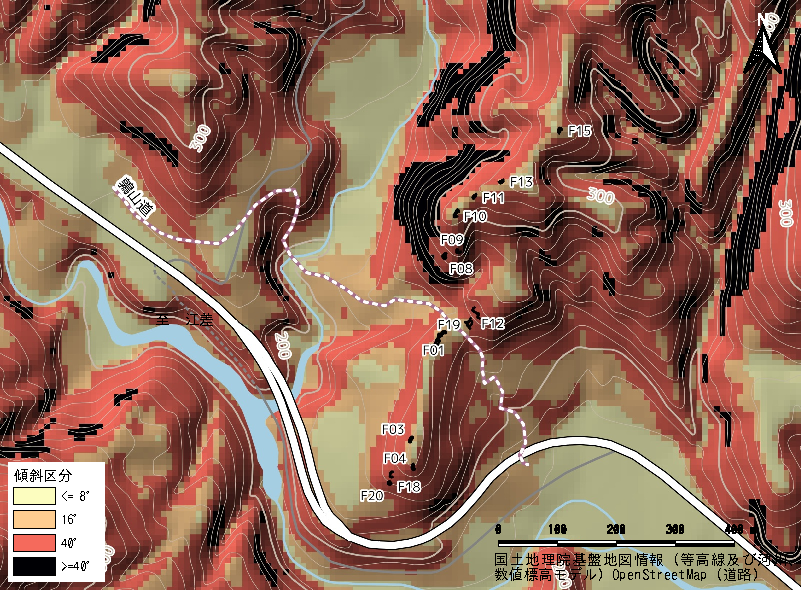
\includegraphics[width=160truemm]{../02fig/03slope.pdf}
\caption{二股台場の塹壕配置と地形}
\label{slope}
\end{figure}

%%%%
\section{主な塹壕}

\begin{figure}[ht]
\centering
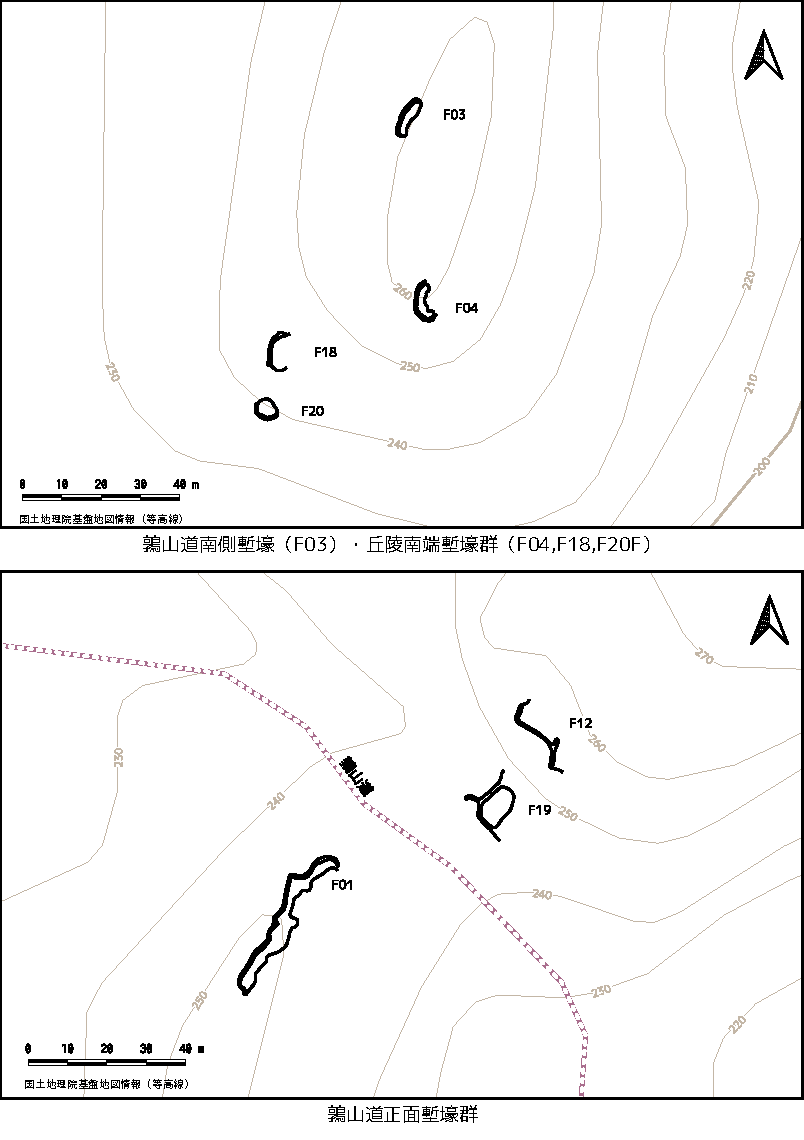
\includegraphics[width=160truemm]{../02fig/04zangou01.pdf}
\caption{塹壕配置図(1)}
\label{zangou01}
\end{figure}

\begin{figure}[ht]
\centering
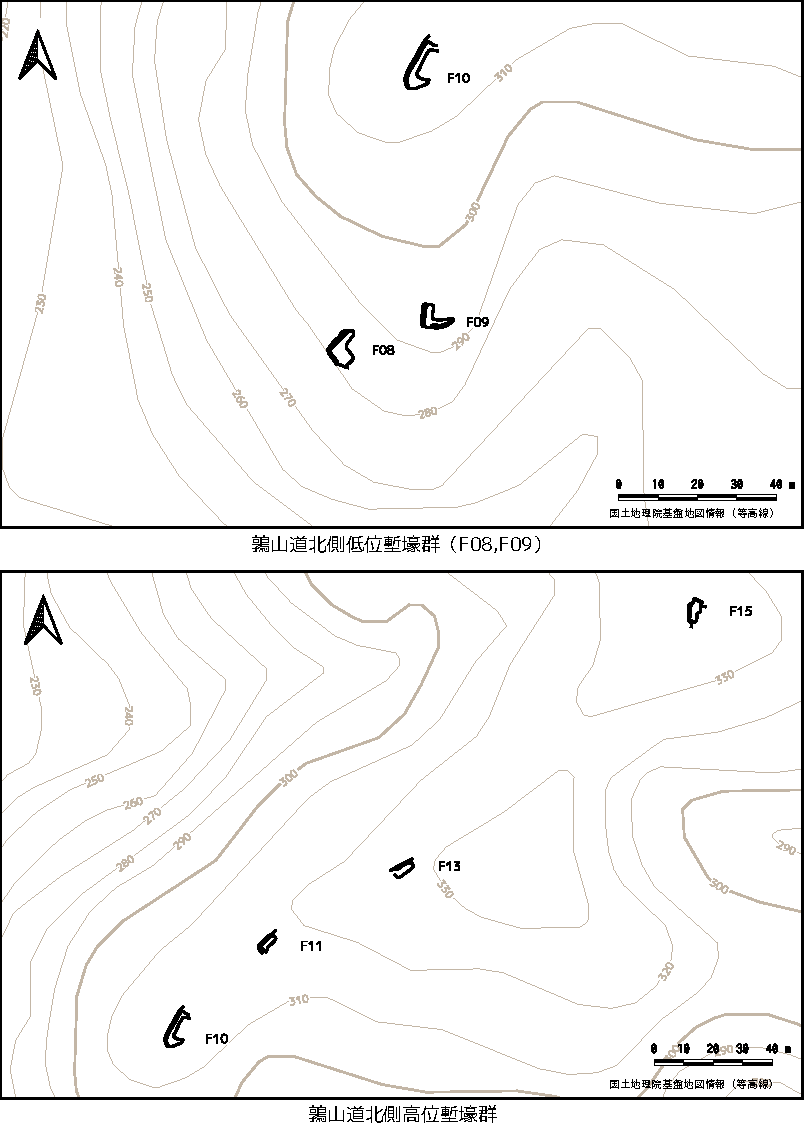
\includegraphics[width=160truemm]{../02fig/05zangou02.pdf}
\caption{塹壕配置図(2)}
\label{zangou02}
\end{figure}

\subsection{丘陵南端塹壕群(図\ref{zangou01}上)}
\subsubsection*{形状}
F04、F18、F20がある。いずれも西または南側に土塁をもつ。

F04は下端延長8.7m、下端幅0.9mの馬蹄形で、土塁は北西から南向きに設けられる。

F18は長軸7.3m、短軸3.2m、溝状ではなく、幅の広い平坦面をもつ。北西と西に土塁が設けられる。

F20は下端延長3.3m、下端幅1.1mである。土塁は西から南東向きの馬蹄形となる。

\subsubsection*{考察}
 丘陵南端塹壕群を構成する塹壕のうち、F04は尾根上に位置し、3つの塹壕のうち最高所にある。F18及びF20 を俯瞰できる位置にあることから、F04支援のため、陣地を前進させF18及びF20が構築されたものと推測できる。F18とF20は隣接して構築されており、直接的なコミュニケーションが可能な位置関係にある。戦闘時には、最高所のF04から広域の戦況を把握し、F18、F20を前進陣地として3つの塹壕が連携して機能したものと推測する。

%%%
\subsection{鶉山道南側塹壕群(図\ref{zangou01}上)}
\subsubsection*{形状}
F03の1箇所のみが確認されている。

下端延長8.7m、下端幅1.2mの馬蹄形で土塁は西に設けられる。

\subsubsection*{考察}
鶉山道南側に位置するF01からF03までは直線距離で148mあり、この間には塹壕が検出されていない。F03正面は傾斜角10度未満の緩斜面が広がり、二股台場の中でもっとも地形的に攻略が容易な箇所となっている。それにもかかわらずF01を含めて2箇所しか塹壕が確認されていないことは、未検出の塹壕があると考えるのが自然であろう。

%%%
\subsection{鶉山道正面塹壕群(図\ref{zangou01}下)}
\subsubsection*{形状}
F01、F12、F19がある。北西または南西に土塁が設けられる。

F01は鶉山道南側に位置し、下端延長42m、下端幅1.8m〜2.8mである。突出部が2〜3箇所みられることから「イナズマ形」と呼称されることも多い。後世の踏み跡によって、本来2つだった塹壕間が溝状に連結した可能性もある。

F12は鶉山道北側でF19を俯瞰する位置にある。掘り込みは不明瞭で「S」字状の土塁が確認できる。土塁の延長は20.4mである。土塁は南西と北西に設けられる。

F19は鶉山道北側に位置し、鶉山道に隣接する。長軸7.8m、短軸3.8mの長方形の掘り込みをもち、北西と南西に土塁を設ける。

\subsubsection*{考察}
新政府軍の攻撃路にあたる鶉山道正面に位置することから、複雑で規模の大きな塹壕で構成される。F19は長方形の竪穴であることから、他の塹壕とは異なり、内部に建物が設置されていた可能性もある。F12はF19の山側直上の平坦面に位置しておりF19を支援しつつF01とともに鶉山道に対して抑止力を発揮していたものと考える。

%%%
\subsection{鶉山道北側低位塹壕群(図\ref{zangou02}上)}
\subsubsection*{形状}
鶉山道正面塹壕群や鶉山道南側塹壕群とは谷を挟んで別の尾根筋に位置する。西側から南側にかけては傾斜40度以上の急斜面である。本塹壕群は25度前後の斜面に立地する。北西から南に土塁が設けられる。

F08はL字形で下端延長9.0m、下端幅は南側で2.1m、北側で0.6mである。土塁は北西と南西に設けられる。

F09はL字形で下端延長9.9m、下端幅0.6mである。土塁は西側と南側に設けられる。

\subsubsection*{考察}
本塹壕群の所在する鶉山道北側尾根は、鶉山道正面塹壕群の手前に張り出すように位置する。本塹壕群の西側及び南側斜面は40度以上の急傾斜となっており、この方向からの攻略は極めて困難である。本塹壕群は二股沢川方面からの攻撃に対する優位を確保しつつ、鶉山道正面塹壕群及び鶉山道南側塹壕群を攻略する敵を側射する位置を選地したものと考える。

%%%
\subsection{鶉山道北側高位塹壕群(図\ref{zangou02}下)}
\subsubsection*{形状}
鶉山道北側低位塹壕群上位の尾根上に分布する。F10、F11、F13、F15の4箇所を確認した。いずれも北西に土塁をもつ。F10、F11、F13 は約50m間隔で尾根上に塹壕が並ぶ。F13からF15の間はピークと鞍部を挟んで130mの距離があるが、この間に塹壕を確認することはできなかった。

F10は下端延長13.4m、下端幅0.6mでコの字状となる。土塁は北西側に設けられる。

F11は下端延長4.9m、下端幅0.9m、南西端が直角に屈曲しL字状となる。土塁は北西側と南西側に設けられる。

F13は下端延長6.4m、下端幅0.8m、直線的な形状である。土塁は北西側に設けられる。

F15は下端延長6.0m、下端幅2.0mである。高圧電線保線用作業道が塹壕を横断しており、土塁の一部が破損している。北と西に土塁が設けられる。

\subsubsection*{考察}
本塹壕群は鶉山道北側の高位の尾根上に位置する。いずれも、二股川方向に土塁を有する。本塹壕群の位置からは鶉山道は視認できず、鶉山道低位塹壕群やその他の塹壕群と直接的な支援を行い得る位置関係にはない。二股川対岸の敵の動きを牽制し、二股川上流を迂回しようとする動きを妨害する目的で構築されたものと推測する。


%%%%
\section{塹壕群の可視領域}

\begin{figure}[ht]
\centering
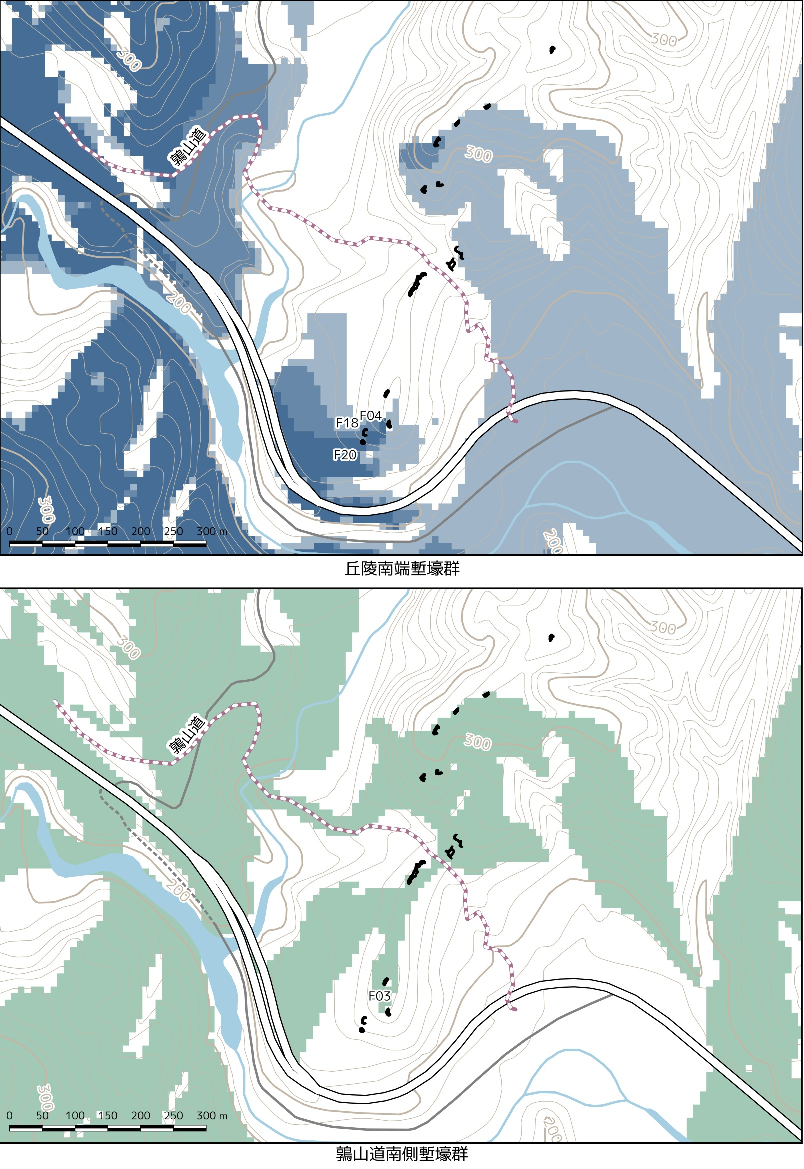
\includegraphics[width=160truemm]{../02fig/08view01.pdf}
\caption{塹壕群の可視領域(1)}
\label{view01}
\end{figure}

\begin{figure}[ht]
\centering
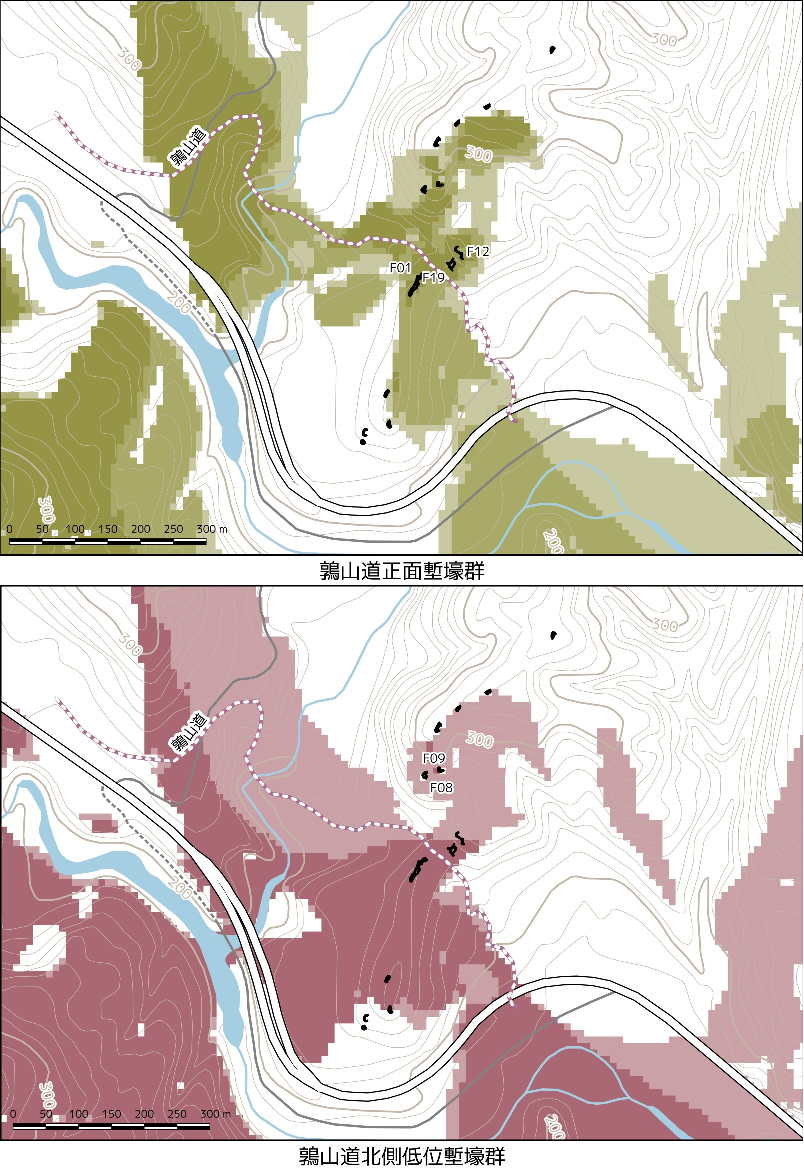
\includegraphics[width=160truemm]{../02fig/09view02.pdf}
\caption{塹壕群の可視領域(2)}
\label{view02}
\end{figure}

\begin{figure}[ht]
\centering
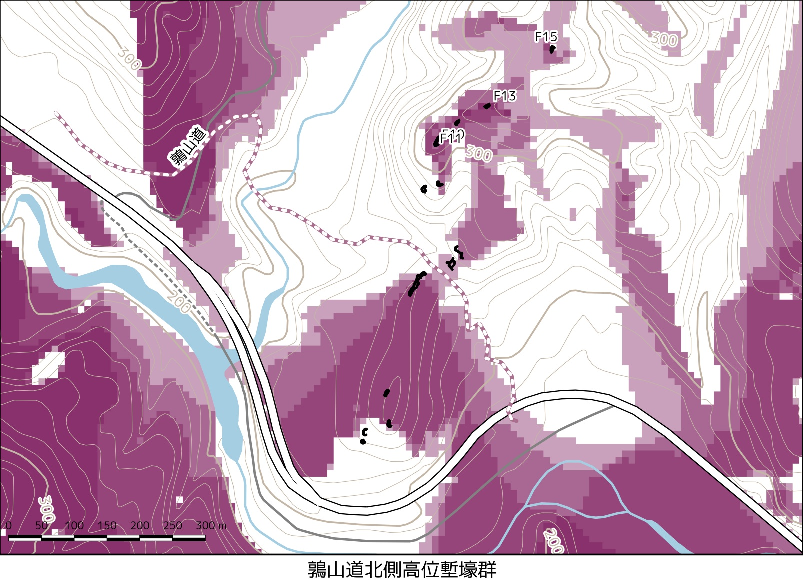
\includegraphics[width=160truemm]{../02fig/10view03.pdf}
\caption{塹壕群の可視領域(3)}
\label{view03}
\end{figure}


\subsection{可視領域の算出}
可視領域の算出起点は各塹壕下端の平面上の重心座標とした。可視領域の算出にはGRASS GISの「r.viewshed」コマンドを利用し、可視領域算出の基準となる地上高は1.75mとした。算出された可視領域をベクタ化し、汎用性の高いフォーマット(shape形式)に出力した。

%%%
\subsection{塹壕群の可視領域}
\subparagraph{丘陵南端塹壕群}
南西側に可視領域が広がり、攻撃正面となる鶉山道や鶉山道南側尾根の西面には視界が効かない(図\ref{view01}上)。

\subparagraph{鶉山道南側塹壕群}
主な可視領域は鶉山道南側丘陵の西面緩斜面である。鶉山道にもわずかに視界が効くが、300m以上離れている(図\ref{view01}下)。

\subparagraph{鶉山道正面塹壕群}
鶉山道上に可視領域が重複する。鶉山道南側丘陵西側の緩斜面にも一部視界が効く(図\ref{view02}上)。

\subparagraph{鶉山道北側低位塹壕群}
鶉山道及び鶉山道南側丘陵の西面に可視領域が広がる(図\ref{view02}下)。

\subparagraph{鶉山道北側高位塹壕群}
鶉山道にはほとんど視界が効かず、鶉山道南側丘陵の一部に視界が効くが、尾根頂部が中心となる。鶉山道北側高位塹壕群の可視領域の大部分は二股沢川対岸に広がる(図\ref{view03})。

%%%
\subsection{考察}
\subparagraph{丘陵南端塹壕群}
攻撃正面と想定される鶉山道や鶉山道南側丘陵西面に視界が効かず、丘陵の南西部に可視領域が集中することから、これらの塹壕は、二股台場を大野川に沿って南側から迂回されることを阻止する機能を担ったと推測する。

\subparagraph{鶉山道南側塹壕群}
現時点ではF03しか確認されていないため断定は避けたいが、二股沢川方向に広く視界が効き、一部鶉山道も可視領域に含まれることから、丘陵西面の緩斜面からの攻撃に備えることを主目的とし、鶉山道を側射する機能も併せもつと推測する。

\subparagraph{鶉山道正面塹壕群}
3つの塹壕の可視領域が鶉山道上で重複することから、鶉山道を侵攻する敵を正面から封殺することがその主たる機能と推測する。また、鶉山道南側丘陵西面にも一部視界が効くことから、丘陵南側の西面を側射する機能もあったと推測する。

\subparagraph{鶉山道北側低位塹壕群}
鶉山道と鶉山道南側丘陵西面全域に視界が効くことから、鶉山道とその南側の西斜面に対して側射することが主な機能と推測する。

\subparagraph{鶉山道高位塹壕群}
主戦場となる鶉山道や鶉山道南側丘陵西面には視界が効かず、主に二股沢川対岸に視界が効くことから、これらの塹壕群二股沢川対岸の新政府軍陣地での活動や北側からの迂回を監視・牽制することが主な機能と推測する。

%%%%
\section{まとめ}
\subsection{二股台場の立地}
函館側からみた場合、二股台場は急峻な山道の開始地点にあたる。これより下流では大野川沿いに平坦地を通行することとなる。一方、江差側からみた場合、二股台場は長い山道の終端に位置することとなる。二股台場の立地は、旧幕府軍補給線の負担を軽減しつつ、新政府軍には最大限の負担を強いる地理的環境となっている。

第一次会戦の後、新政府軍は厚沢部稲倉石まで撤退を余儀なくされているが、二股台場から稲倉石までは現在の国道227号を基準としても山中を14km以上の距離となる。旧幕府軍の補給拠点は市渡村(現北斗市一渡)と考えられるが、約10kmの平坦地の補給線であり、両軍の補給格差は大きいと推測する。新政府側の記録にも「雨は降し非常な困難で、食料も来ない」、「度々稲倉市(「稲倉石」:執筆者註)まで休養の為に戻らなければならぬので不便でいけません」(児玉恕忠「函館役」)とあり、補給に困難を生じていたことを示す描写がある。

%%%
\subsection{塹壕配置からみる旧幕府軍の防衛構想}

\begin{figure}[ht]
\centering
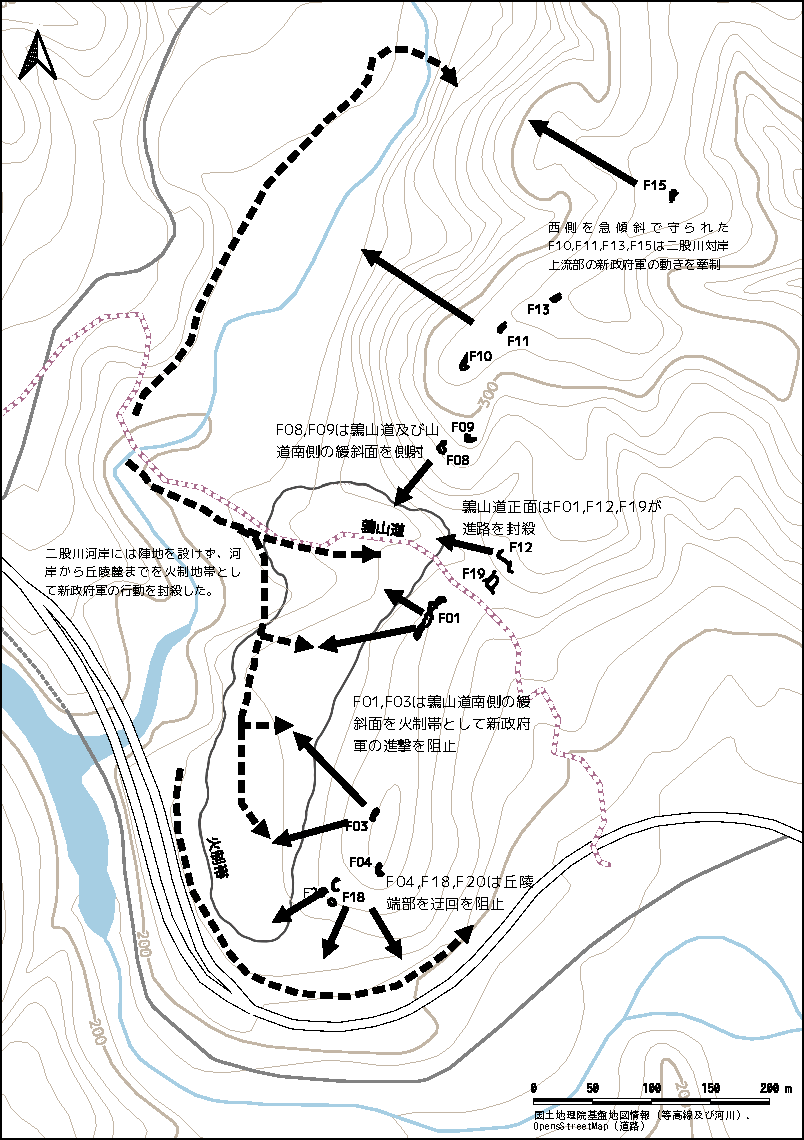
\includegraphics[width=160truemm]{../02fig/11battle_model.pdf}
\caption{二股台場戦闘模式図}
\label{battle}
\end{figure}

二股台場は鶉山道とその南側尾根では傾斜が緩く、地形的には攻略が容易である。一方、鶉山道北側尾根の西面は、一部に岩肌が露出する40度以上の急傾斜となっている。このため、二股沢川方面から直接的に鶉山道北側尾根を攻略することは困難である。旧幕府軍は、この北側尾根に塹壕を配置し、防御正面となる鶉山道や鶉山道南側の緩斜面を側射できるようにしたのである。鶉山道を封殺する鶉山道正面塹壕群を開口部とみた場合、その前面に張り出す北側尾根は「食い違い虎口」のような位置関係となっており、鶉山道正面塹壕群に接近する敵を、側面又は背面から攻撃することが可能となっている。こうした、自然地形の活用が二股台場を構成する重要な要素となったと考える。

一方、鶉山道南側では二股沢川河岸から尾根の麓までは幅約100mの平坦地が広がる。一見たやすく侵攻できそうだが、尾根上の塹壕群や鶉山道北側塹壕群からの十字砲火を受ける火制帯となっている。旧幕府軍は二股沢川河岸に塹壕を設けていたようだが、河岸を阻止線とはせず、主陣地は尾根上に設け、二股河岸から尾根までの平坦地を陣前地として火力の集中が可能となる塹壕配置を実現した。このことで、新政府軍は開平地での長距離突撃を強いられる結果になったと解釈できる。地形的に攻略の容易な鶉山道南側の尾根に向かった新政府軍に対して、鶉山道南側塹壕群や鶉山道正面塹壕群からの正面射撃と鶉山道北側塹壕群からの側面射撃が組み合わされ、新政府軍は遮るもののない平坦地で十字砲火を浴びることになったと推測される(図\ref{battle})。

%%%
\subsection{結論}
二股台場をめぐる攻防戦では小銃が主兵器として用いられた。旧幕府軍ではミニエー銃弾を使用する前装式施条銃、新政府軍ではこれに加えて後装式施条銃が用いられた。これらの施条銃の銃撃開始距離は「300メートル弱から500メートルくらい」とされ(保谷2007: 215)、滑腔銃に比較して、射程距離と命中精度が大幅に向上し、散開戦闘が歩兵部隊の基礎的な戦術様式となった(保谷 2013)。二股台場の攻防は、明治元年の戦争を通して施条銃を用いた戦闘を経験し、戦闘技術を蓄積した部隊同士の戦闘である。防御側の旧幕府軍は、尾根上に塹壕を散在させ、それらを効果的に組み合わせて防御戦を構想していたことが明らかである。二股台場ではそのような戦闘技術の運用の痕跡が塹壕群として保存されている。

これらの塹壕群は当初の作戦構想として準備構築されたものと、戦闘経過において包囲と内旋のプロセスとして構築されたものがあると考えられる。今回の調査では、そのような経時的なプロセスを復元することはできなかったが、施条銃の特性を生かした陳地構築を、正面防御と側面射撃を塹壕群の組み合わせによって実現しようとした築城主体の意図を読み解くことができた。

%%%%
\subsection*{謝辞}
筆者らの調査成果は、函館市在住毛利剛氏の踏査成果によるところが大きい。毛利氏は塹壕の図化とともに、GPSで取得した位置情報を公開している。これらの情報を頼りに筆者らは円滑に調査を進めることができた。毛利氏の丹念なフィールドワークと適切な記録の公開に敬意と感謝の意を表するとともに、学術調査の手本として引き継いでいきたい。

%%%%
\subsection*{翻刻}
参照した翻刻は次の通りである。

\mbox{}\\ 
『南柯紀行』、『蝦夷之夢』(大鳥ほか 1988)\\
『新開調記』、『説夢録』、『衝鋒隊戦争略記』、『北洲新話』、『苟生日記』、『蝦夷錦』、『戊辰戦争見聞略記』、『星恂太郎日記』、『函館戦記』(須藤隆仙編 1996)\\
『中島登覚え書』、『島田魁日記』、『立川主税戦争日記』、『函館戦記』(大野右仲)(新人物往来社編 1995)\\
『新選組史料集』(新人物往来社編 1995)\\
『戦争御届書』( 松前町史編集室編1974 )\\
『戊巳征戦記略』、『山口藩忠節事蹟』、『岡山藩記』、『阿部正桓家譜』、『討北紀略』、『弘前藩記』、『津軽承昭家記』、『毛利元功家記』、『蝦地征討録』、『太政官日誌』(太政官編 1930)\\
『薩藩出軍戦状』(大塚武松編 1932-1933)\\
『維新戦役実録談』(維新戦歿者五十年祭事務所編 1917)\\

%%%
\subsection*{引用文献}
\vspace{-1\baselineskip}
\mbox{}\\ 
維新戦歿者五十年祭事務所編 1917 『維新戦役実録談』 維新戦歿者五十年祭事務所\\
大鳥圭介・今井信郎編著 1998 『南柯紀行・北国戦争概略衝鉾隊之記』 新人物往来社\\
大塚武松編 1932-1933 『薩藩出軍戦状』第二 日本史籍協会\\
河野常吉 1924『北海道史蹟名勝天然記念物調査』 北海道立図書館所蔵,1974年復刻版『北海道史蹟名勝天然記念物調査』名著出版 88-91\\
新人物往来社編 1995『新選組史料集』 新人物往来社\\
須藤隆仙編 1996 『箱館戦争史料集』 新人物往来社\\
太政官編 1929 『復古記』第14冊 内外書籍\\
保谷徹 2007 『戊辰戦争(戦争の日本史)』18 吉川弘文館\\
保谷徹 2013 「施条銃段階の軍事技術と戊辰戦争」 箱石大編『戊辰戦争の史料学』 勉誠出版 61-87\\
松前町史編集室 1974 「戦争御届出書」『松前町史(史料編)』第1巻 松前町 317-343\\
毛利 剛 2012 『二股口台場』自遊出版工房\\

\end{document}  
